\begin{figure}[ht]
    \centering
    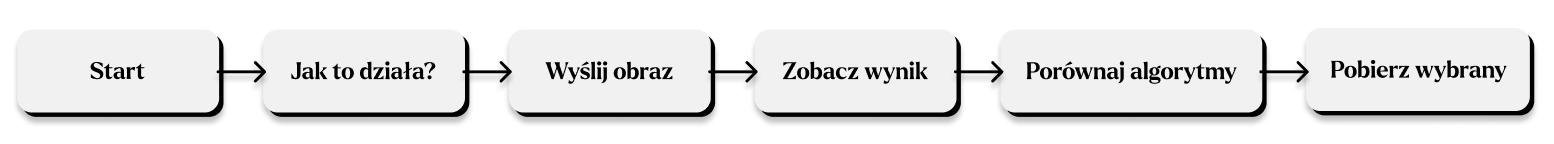
\includegraphics[width=\linewidth]{Rozdziały/06.Aplikacja/Obrazy/user-flow.png}  
    \caption{Diagram przepływu użytkownika}
    \label{fig:image82}
\end{figure}

TODO: Usuń diagram przepływu

\section{Implementacja aplikacji}

Po wyborze stosu technologicznego kolejnym krokiem jest skupienie się na implementacji rozwiązań. W tym rozdziale opiszę jakie decyzje podjąłem przy pisaniu kodu aplikacji, jak wygląda jej struktura i jakie problemy napotkałem podczas implementacji.

\subsection*{Struktura aplikacji}

Aplikacja składa się z dwóch części - Frontendu i Backendu. Przy tworzeniu takiego projektu warto zadbać o to, żeby każda część była od siebie niezależna i żeby komunikacja między nimi była jak najmniej skomplikowana.

W tym miejscu wracamy do diagramu przepływu użytkownika [Rys \ref{fig:image82}], jak na nim widać użytkownik nie może wykonać zbyt wiele akcji, struktura aplikacji jest liniowa. Na podstawie diagramu przepływu użytkownika można stworzyć schemat blokowy aplikacji [Rys \ref{fig:image87}], który pozwoli zrozumieć zachowanie programu.

\begin{figure}[H]
    \centering
    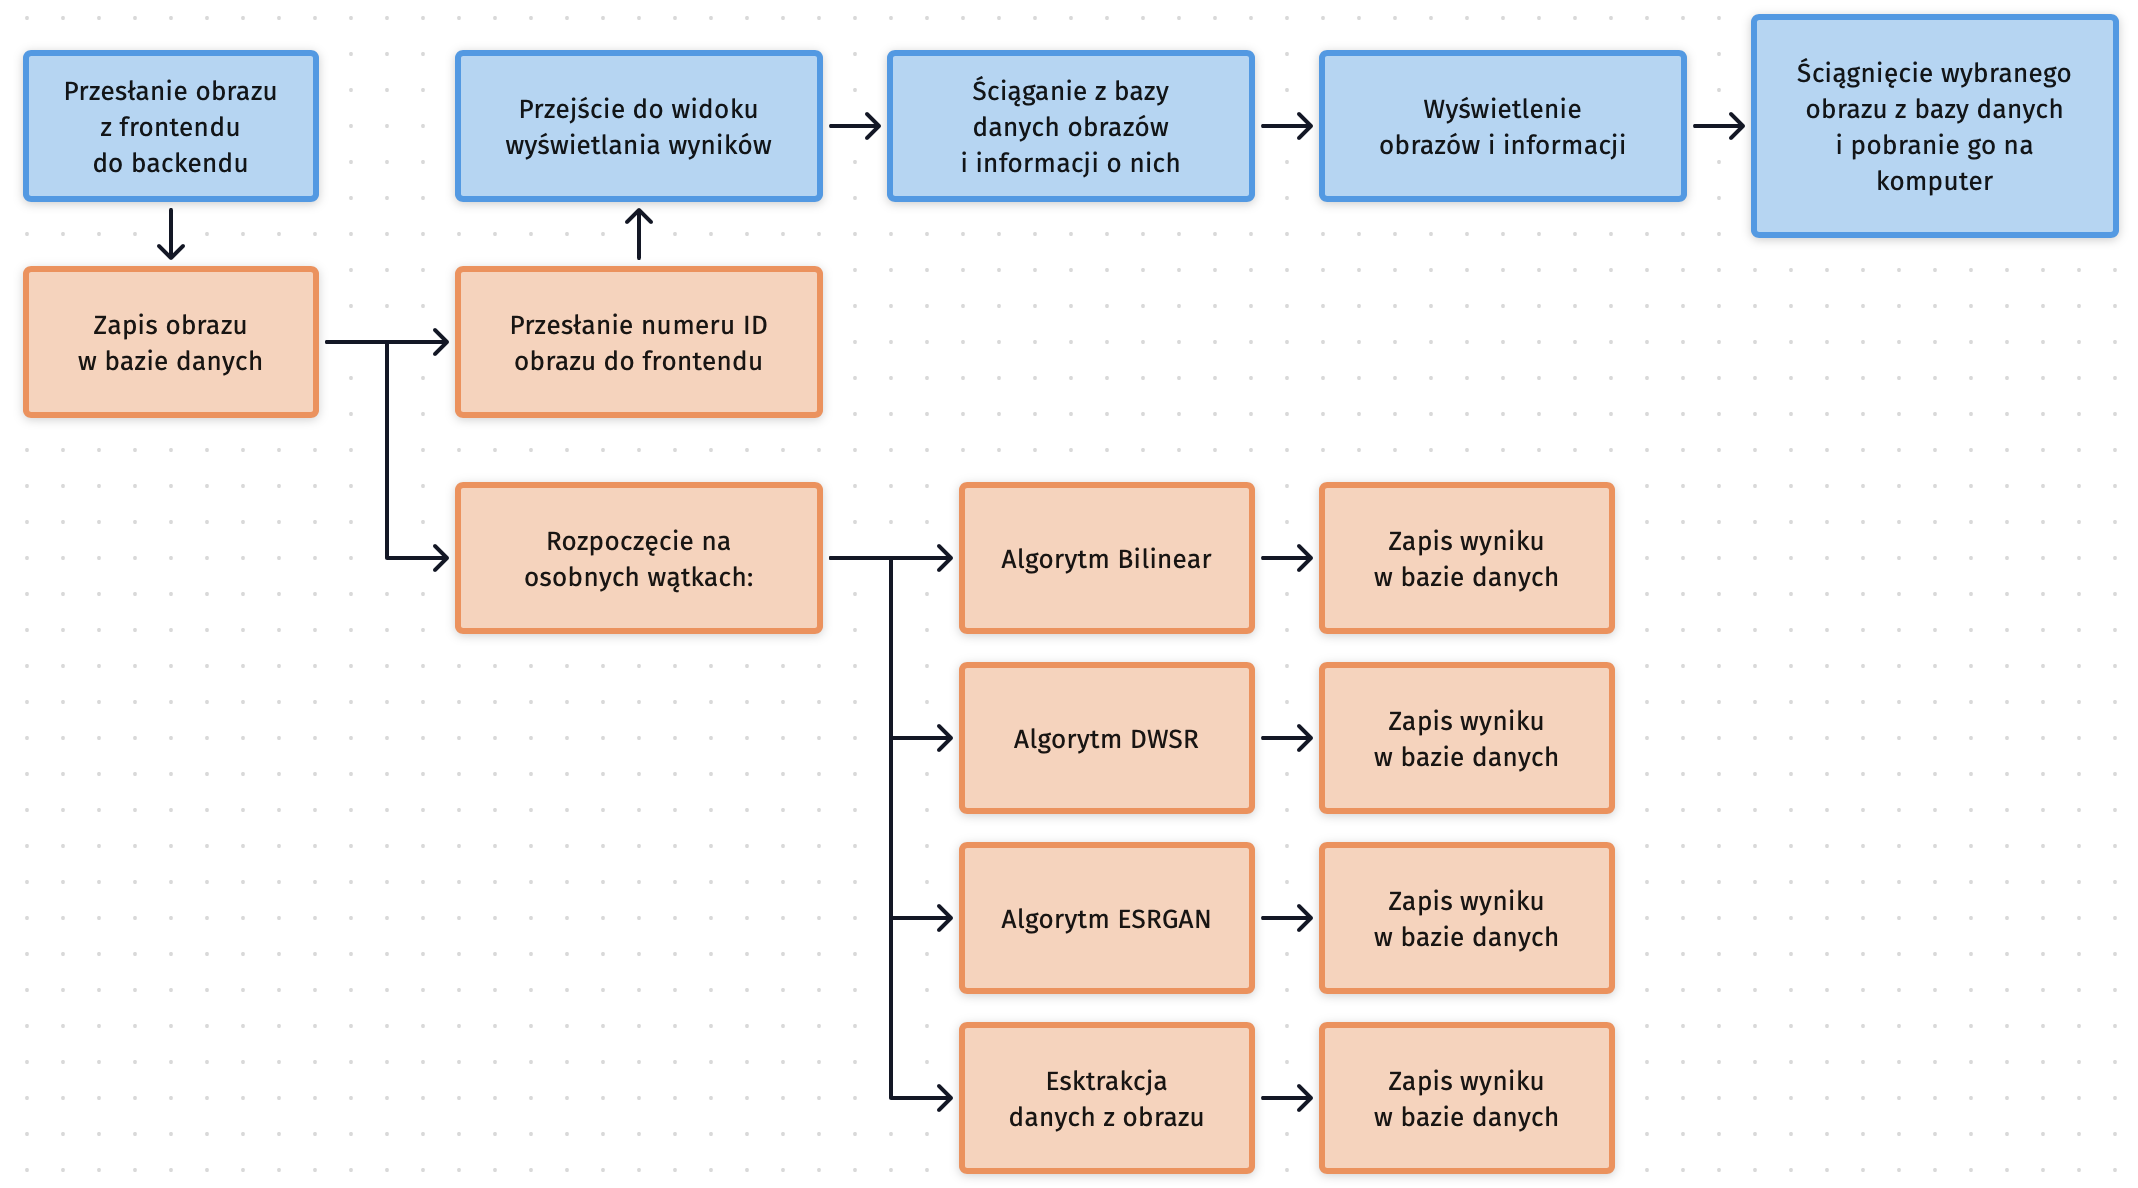
\includegraphics[width=\linewidth]{Rozdziały/06.Aplikacja/Obrazy/mechanizm_aplikacji.png}  
    \caption{Schemat blokowy aplikacji (kolor niebieski - Frontend, pomarańczowy - Backend)}
    \label{fig:image87}
\end{figure}

W pierwszej kolejności użytkownik wysyła obraz do serwera Backend, który zapisuje go w bazie danych. Następnie serwer zleca wykonanie algorytmów na osobnych wątkach, o czym opowiem w dalszej części rozdziału [\ref{sec:implementation-s-r}]. Gdy algorytmy rozpoczną pracę, serwer zwraca do Frontendu informację o tym że operacja zapisu się powiodła i podaje numer ID obrazu. 

Frontend zmienia widok na ten z wynikami i wysyła zapytanie do Backendu o obraz oryginalny i przetworzone. Następnie jeśli serwer zwróci obrazy, Frontend je wyświetla. W przeciwnym wypadku próbuje je pozyskać ponownie aż do skutku. Dzieje się tak, dlatego że zadanie super-rozdzielczości jest czasochłonne i czasem może zająć kilka sekund a w innych wypadkach nawet kilka minut, wszystko w zależności od rozdzielczości obrazów. W tym czasie użytkownik może porównywać uzyskane wyniki i wybrać najlepszy. 

Gdy użytkownik wybierze obraz, może go pobrać na swój komputer. Wtedy Frontend wysyła zapytanie do serwera o obraz w pełnej rozdzielczości, a serwer zwraca obraz, który przeglądarka automatycznie pobiera.

\subsubsection*{Architektura bazy danych}

Baza danych w aplikacji jest bardzo prosta, przy przesłaniu każdego zdjęcia w bazie tworzone jest pole Image, które przechowuje informacje o obrazie oraz jego przetworzonych wersjach. W tabeli \ref{tab:image_model} przedstawiam jedyną tabelę w bazie danych, która przechowuje informacje o obrazach.

\begin{table}[ht]
    \centering
    \renewcommand{\arraystretch}{1.5} % Increase row height by 1.25 times
    \begin{tabular}{|l|l|p{8cm}|}
    \hline
    \multicolumn{3}{|c|}{\textbf{Image}}                                                        \\ \hline
    \textbf{Pole}       & \textbf{Typ}          & \textbf{Opis}                                 \\ \hline
    image               & ImageField            & Przesłany obraz.                              \\ \hline
    bilinear\_image     & ImageField            & Obraz powiększony algorytmem Bilinear.        \\ \hline
    dwsr\_image         & ImageField            & Obraz powiększony algorytmem DWSR.            \\ \hline
    esrgan\_image       & ImageField            & Obraz powiększony algorytmem ESRGAN.          \\ \hline
    original\_height    & PositiveIntegerField  & Wysokość oryginalnego obrazu.                 \\ \hline
    original\_width     & PositiveIntegerField  & Szerokość oryginalnego obrazu.                \\ \hline
    dominant\_colors    & TextField             & Pole tekstowe z listą dominujących kolorów.   \\ \hline
    \end{tabular}
    \caption{Struktura bazy danych - Image.}
    \label{tab:image_model}
\end{table}

Jak widać w bazie danych przechowywane są obrazy w formacie \textit{ImageField}, który jest dostarczany przez bibliotekę Django. Jest to pole, które przechowuje ścieżkę do pliku na dysku serwera. Zapisujemy również informacje o oryginalnych wymiarach obrazu, które są wyświetlane użytkownikowi przez Frontend. 

Dodatkowo w bazie danych przechowujemy listę dominujących kolorów, które są wykrywane przez algorytm K-średnie \textit{K-means}, o którym opowiem w kolejnym rozdziale [\ref{sec:implementation-s-r}]. Jest to lista kolorów w formacie HEX, które wykorzystuje Frontend do wyświetlenia kolorowych gradientów tła.


\newpage
\section{Integracja algorytmów super-rozdzielczości} \label{sec:implementation-s-r}

Gdy obraz jest już zapisany w bazie danych, serwer Backend zleca wykonanie algorytmów super-rozdzielczości na osobnych wątkach [\ref{lst:save_image}]. W tym rozdziale opiszę w jaki sposób zostały zaimplementowane algorytmy w aplikacji.

\begin{lstlisting}[language=Python, caption=Obsługa zapisu i przetwarzania obrazów., label={lst:save_image}]
def upload_image(request):
try:
    form = Image(image=request.FILES['image'])
    form.save()

    input_image_path = form.image.path
    
    thread1 = threading.Thread(target = run_bilinear, 
                                args = (input_image_path, 4, form))
    thread2 = threading.Thread(target = run_dwsr, 
                                args = (input_image_path, 4, form))
    thread3 = threading.Thread(target = run_esrgan, 
                                args = (input_image_path, form))
    thread4 = threading.Thread(target = extract_image_info, 
                                args = (input_image_path, form))
    thread1.start()
    thread2.start()
    thread3.start()
    thread4.start()

    image = Image.objects.latest('id')  # Gets the latest entry

    return JsonResponse({'message': 'Image uploaded, processing started', 
                            'image_id': image.id})
except Exception as e:
    return JsonResponse({'error': str(e)}, status=400)
\end{lstlisting}

Stworzone zostały cztery funkcje - \textit{run\_bilinear}, \textit{run\_dwsr}, \textit{run\_esrgan} oraz\\ \textit{extract\_image\_info}. Pierwsze trzy z nich odpowiadają za uruchomienie algorytmów super-rozdzielczości, a ostatnia za wydobycie informacji o obrazie.




\subsection*{Algorytm Interpolacji Dwuliniowej}

Pierwszy z algorytmów, który został zaimplementowany to algorytm Interpolacji Dwuliniowej omawiany w rozdziale
TODO: Końcowe: Daj ref do podstaw teoretycznych Bilinear.
Jest to najmniej skomplikowany algorytm, więc implementacja jego nie była trudna [\ref{lst:bilinear}].

\begin{lstlisting}[language=Python, caption=Implementacja algorytmu Bilinear., label={lst:bilinear}]
def run_bilinear(input_image_path, scale, image_instance):
    img = cv2.imread(input_image_path, cv2.IMREAD_COLOR)
    
    height, width = img.shape[:2]
    new_width, new_height = width * scale, height * scale

    # Resize the image using bilinear interpolation
    output = cv2.resize(img, (new_width, new_height), interpolation=cv2.INTER_LINEAR)

    save_output_image(output, input_image_path, image_instance)
\end{lstlisting}

W pierwszej kolejności wczytujemy obraz do powiększenia, następnie pobieramy jego wymiary i mnożymy je przez skalę powiększenia otrzymując nową wielkość obrazu. W kolejnym kroku wykorzystujemy funkcję \textit{cv2.resize} z biblioteki OpenCV2, która pozwala na zmianę rozmiaru obrazu. W tym miejscu wykorzystujemy parametr \\ \textit{interpolation=cv2.INTER\_LINEAR}, który odpowiada za wybór algorytmu interpolacji. W tym wypadku wybraliśmy algorytm Interpolacji Dwuliniowej. Na koniec zapisujemy obraz w bazie danych.


\subsection*{Algorytm DWSR}

Kolejnym algorytmem jest algorytm DWSR, który został opisany w rozdziale 
TODO: Końcowe: Daj ref do DWSR.
Implementacja tego algorytmu jest bardziej skomplikowana, ponieważ wymaga on zainstalowania modelu, który jest wykorzystywany do przetwarzania obrazów, oraz wymagała przepisania skryptów napisanych w Matlabie na język Python [\ref{lst:dwsr}].


\begin{lstlisting}[language=Python, caption=Implementacja algorytmu DWSR., label={lst:dwsr}]    
def run_dwsr(input_image_path, scale, image_instance):
    enlarged_lr_dir, sr_lum_dir, output_dir = create_output_dir()

    fileName = os.path.basename(input_image_path)

    # 1. Generate enlarged LR images
    generate_enlarged_lr(input_image_path, enlarged_lr_dir, scale) 

    # 2. Process image with DWSR
    process_image(enlarged_lr_dir + '/' + fileName, sr_lum_dir, scale)

    # 3. Generate color SR
    final_img_path = generate_color_sr(input_image_path, sr_lum_dir, 
                                       output_dir, scale) 

    save_output_image(final_img_path, input_image_path, image_instance)
\end{lstlisting}

Algorytm DWSR składa się z trzech etapów, najpierw obraz jest powiększany metodą Bicubic o podaną skalę analogicznie do algorytmu Bilinear, lecz tym razem z parametrem \textit{interpolation=cv2.INTER\_CUBIC}. Obraz konwertowany jest do skali szarości. Następnie obraz jest przetwarzany przez model DWSR [\ref{lst:dwsr_2}], który zwraca obraz w skali szarości. Na koniec obraz jest konwertowany do RGB i zapisywany w bazie danych.


\begin{lstlisting}[language=Python, caption=Przetwarzanie przez model DWSR., label={lst:dwsr_2}]    
def process_image(input_image_path, output_dir, scale):
    session = initialize_session()

    coeffs = dwt2_image(input_image_path)
    model_input_data = construct_model_input(coeffs)

    model_output_data = session.run([model_output], 
                        feed_dict={model_input_data})
    
    super_res_image = idwt2_image(model_output_data)

    output_image_path = os.path.join(output_dir, 
                        ntpath.basename(input_image_path))
    cv2.imwrite(output_image_path, super_res_image)        
    session.close()

\end{lstlisting}

Przetwarzanie obrazu przez model DWSR rozpoczyna się od załadowania wytrenowanego modelu i obrazu powiększonego przez Bicubic. Następnie obraz jest dekomponowany na współczynniki falkowe (z użyciem biblioteki PyWavelets), które są przekształcane do formatu odpowiedniego dla modelu. Model prognozuje ulepszone detale tych współczynników. 
Te przewidziane detale są następnie łączone z oryginalnymi współczynnikami, tworząc obraz o wyższej rozdzielczości. Wynikowy obraz jest zapisywany w tymczasowej lokalizacji a w kolejnym kroku jest on konwertowany ze skali szarości do RGB i zapisywany w bazie danych.


\subsection*{Algorytm ESRGAN}

Ostatnim algorytmem Super-Rozdzielczości implementowanym w aplikacji jest algorytm ESRGAN, który został opisany w rozdziale 
TODO: Końcowe: Daj ref do ESRGAN.
Implementacja tego algorytmu była prosta, ponieważ wymagała jedynie zapisu modelu, który jest wykorzystywany do przetwarzania obrazów, oraz jako że model jest już napisany w języku Python, nie było potrzeby przepisywania go na inny język [\ref{lst:esrgan}]. Do tej funkcji nie podajemy skali powiększenia, ponieważ model ESRGAN jest w stanie powiększyć obraz czterokrotnie.

\begin{lstlisting}[language=Python, caption=Implementacja algorytmu ESRGAN., label={lst:esrgan}]    
def run_esrgan(input_image_path, image_instance):
    model, device = initialize_esrgan_model()
    output = process_image_with_esrgan(model, device, input_image_path)
    save_output_image(output, input_image_path, image_instance)
\end{lstlisting}

W pierwszej kolejności wczytujemy model ESRGAN, następnie przetwarzamy obraz przez model [\ref{lst:esrgan_2}] i zapisujemy go w bazie danych.


\begin{lstlisting}[language=Python, caption=Przetwarzanie przez model ESRGAN., label={lst:esrgan_2}]
def process_image_with_esrgan(model, device, input_image_path):
    img_LR = read_img(input_image_path, device)

    with torch.no_grad():
        output=model(img_LR).data.squeeze().float().cpu().clamp_(0, 1).numpy()
    
    output = np.transpose(output[[2,1,0],:,:],(1,2,0))
    output = (output * 255.0).round()
    return output
\end{lstlisting}


\subsection*{Algorytm K-średnich}

Algorytm K-średnich został opisany w rozdziale
TODO: Końcowe: Daj ref do K-średnich.
Jest to algorytm, który wykorzystujemy do wydobycia informacji o obrazie, a dokładniej do wydobycia listy dominujących kolorów. Implementacja tego algorytmu jest bardzo prosta, gdyż wykorzystałem bibliotekę \textit{scikit-learn}, która zawiera w sobie algorytm [\ref{lst:kmeans}].

\begin{lstlisting}[language=Python, caption=Implementacja algorytmu K-średnich., label={lst:kmeans}]
def extract_dominant_colors(input_image_path, image_instance):
    with PILImage.open(input_image_path) as img:
        pixels = np.array(img.getdata())   # Reshape the image data for k-means
        pixels = pixels.reshape(-1, 3)

        kmeans = KMeans(n_clusters=5)
        kmeans.fit(pixels)
        dominant_colors = kmeans.cluster_centers_

        # Convert dominant colors to HEX values
        dominant_colors_list = [rgb_to_hex(tuple(map(int, color))) 
                               for color in dominant_colors]
        image_instance.set_dominant_colors(dominant_colors_list)
        image_instance.save()
\end{lstlisting}

W pierwszej kolejności wczytujemy obraz, następnie przekształcamy go do formatu RGB i przekształcamy do formatu, który może być wykorzystany przez algorytm K-średnich. Następnie wykorzystujemy funkcję \textit{KMeans} z biblioteki \textit{scikit-learn}, która zwraca nam listę dominujących kolorów. Na koniec konwertujemy kolory do formatu HEX i zapisujemy je w bazie danych.

\section{Implementacja interfejsu użytkownika}


\section{Testowanie aplikacji}


\section{Plany na przyszłość} \label{sec:plans}

Opis błędów, rzeczy do poprawy w aplikacji. Omówienie jakie są plany rozbudowy aplikacji.

Przyciski nawigacji z widoku do widoku